\documentclass[a4paper]{article}
\usepackage{graphicx}
\usepackage{hyperref}
\usepackage[inner=0.5cm,outer=0.5cm]{geometry}
\usepackage{mathtools}
\begin{document}

\title{Largest Common Subsequence}
\author{Dmitri Kovalenko}

\maketitle

\section{Code Description}
Main idea behind parallel algorithm design is that every superstep is the processing of one wavefront. Wavefront is such a part of the matrix \textbf{L}, so it's elements lie on the same anti-diagoral layer.  
\subsection{Initialization}
All processing is done by DLargestCommonSubsequence instance. Every process create one of it's own.
Constuctor initalizes set of significant variables like \textit{chunkStride} and \textit{chunkLength}.
Allocation of the respective pieces of matrix \textbf{L}, input strings \textbf{a} and \textbf{b} happens in \textit{distributedInit}.
Also, \textit{distributedInit} allocates vector of rows \textit{over}, which purpose is to be the destination buffer for the last-row communication between processes.
(\textit{*Note} Since current implementation use row-wise allocation of 2d-arrays, \textbf{L} distributed between processes by chunk rows and we trasfer last row between processes, instead of last column, as it was described in article 1.)

\subsection{Distributed Memory}
Chunk is a block of matrix \textbf{L} of size $\textit{chunkLength} \times \textit{chunkLength}$.
Matrix \textbf{L} then could be considered as chunk grid of size $\textit{chunkStride} \times \textit{chunkStride}$. Every chunk could be addressed by pair $[x,y]$ and chunk is owned by  process with $id = x \mod p$.\\
There is a caveat here: for processor \textbf{i} init function allocates not only chunks of $i=x \mod p$ but also last rows of chunks $i-1=x \mod p$. That is done in order to conduct all processing with the data from \textit{L} and to use \textit{over} only for communication.\\
All chunks held by a process are saved in the member map \textit{L}, where key is pair $[x,y]$ and value is data (int**).
\subsection{Processing}
Simplistically described superstep would look like that:
\begin{enumerate}
    \item  (Performed for all wavefronts except the first) For each chunk in this wavefront owned by processor $i$ copy row above this chunk from \textit{over} to \textit{L}. 
    \item Calculate chunk contents
    \item Send last row of every chunk in this wavefront owned by processor $i$ to the \textit{over} buffer of the processor $i+1$.
\end{enumerate}
\section{Analysis}
\begin{align*}
    &  n = \text{problem size}\\
    &  p = \text{processors amont}\\
    &  s = \text{chunk stride} = \alpha  p\\
    &  l = \text{chunk length} = n/s\\
    &  T_{\text{comp}} = (2s-1) \cdot {\frac{n^2}{s^2}} = O(\frac{n^2}{p})\\
    &  T_{\text{comm}} = (2s-1) \cdot l = O(n)\\
    &  T_{\text{sync}} = 2s-1 = O(p)
\end{align*}

\section{Results}
    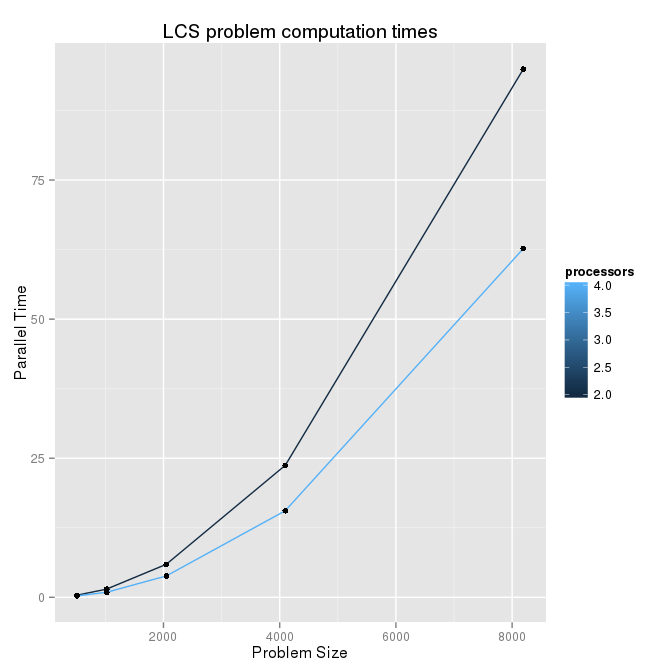
\includegraphics[width=0.45\textwidth]{lcs}
    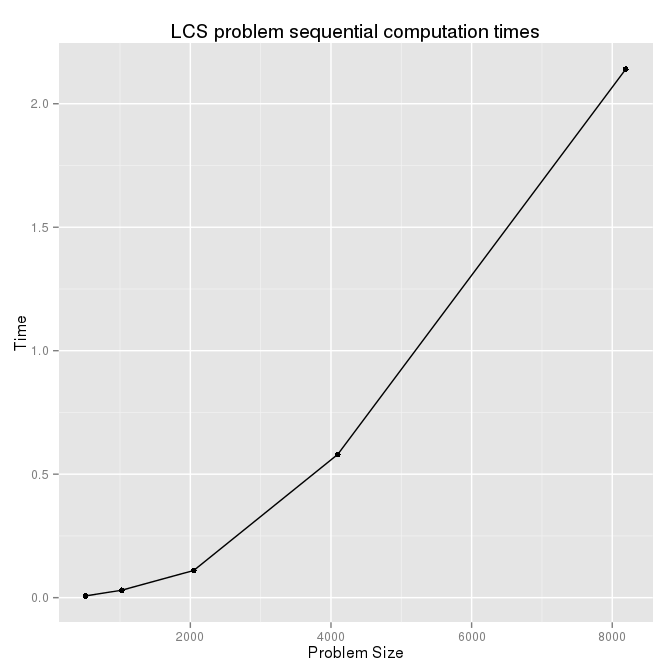
\includegraphics[width=0.45\textwidth]{lcs-seq}

\section{Links}
\begin{enumerate}
    \item Peter Krusche and Alexander Tiskin Efficient Longest Common Subsequence
            Computation using Bulk-Synchronous Parallelism 2006 \url{http://www.dcs.warwick.ac.uk/~tiskin/pub/2006/iccsa.pdf}
  \item  A. Tiskin Advanced Topics in Algorithms \url{http://www2.warwick.ac.uk/fac/sci/dcs/teaching/material/cs341/ata_handout1.pdf}
  \item Peter Krusche and Alexander Tiskin Efficient Parallel String Comparison 2007 \url{http://www.booksonline.iospress.nl/Content/View.aspx?piid=8388}
\end{enumerate}

\end{document}

